% !TEX root = ../main.tex

% ---------------------------------------------------------------
% Background
% ---------------------------------------------------------------

\chapter{Background}\label{chap3:background}
\section{Freezing Of Gait}
Tra i sintomi della malattia di Parkinson, il Freezing può sicuramente essere considerato uno dei più debilitanti. Il Freezing nella malattia di Parkinson, detto anche acinesia paradossa, congelamento o semplicemente blocco motorio, è un’improvvisa, temporanea e involontaria incapacità di iniziare un movimento. È un disturbo che insorge nel corso dell’evoluzione della malattia di cui costituisce un sintomo indipendente e generalmente resistente al trattamento con levodopa. Tale fenomeno si può verificare in ogni momento e i pazienti che lo sperimentano affermano che: \textit{«è come se i piedi rimanessero, per qualche istante, incollati al suolo con la conseguente impossibilità di eseguire il passo successivo»}. In realtà, il Freezing si può verificare anche durante azioni differenti dal cammino come ad esempio l’alzarsi da una sedia o il raccogliere un oggetto. Alcune persone sono più predisposte di altre a subire episodi di congelamento. Tali episodi, si possono verificare sia quando il soggetto è in astinenza da farmaci dopaminergici, in questo caso si parla di “Freezing off”, sia quando il soggetto sta assumendo i farmaci, “Freezing on”. \\
È stato dimostrato che il fenomeno del Freezing nella malattia di Parkinson è spesso collegato alle frequenti cadute a cui i soggetti malati vanno incontro. Le cadute nel Parkinson si verificano più spesso quando il soggetto si gira o cambia direzione e sono frequentemente legate a diversi episodi di Freezing. Non tutti i malati di Parkinson subiscono il fenomeno del Freezing, ma si pensa che coloro che lo provano abbiano una più alta probabilità di cadere a terra. L’imprevedibilità del Freezing, accompagnata dallo sforzo inutile a cui il soggetto si sottopone per cercare di muoversi in avanti, possono causare perdita di equilibrio e quindi cadute. \\
Nel tentativo di superare questo stato di forzata immobilità, i pazienti, talora con un aiuto esterno, cercano di mettere in atto adeguate strategie che si avvalgono di stimoli sensoriali di diversa natura (tattili, visivi oppure uditivi e verbali). Alcune tecniche di tipo motorio o sensoriale possono aiutare i pazienti a convivere con il problema del Freezing. Ad esempio, un paziente incapace di iniziare il primo passo potrebbe riuscire a superare il blocco motorio adottando una delle seguenti strategie:
\begin{itemize}
	\item fare un passo in direzione di un bersaglio;
	\item fare un passo per superare un bastone posto sul pavimento;
	\item fare il primo passo marciando come un soldato.
\end{itemize}
L’idea che sta alla base di tali stratagemmi è mettere in atto un programma motorio volontario che sostituisca il programma motorio automatico malfunzionante nei malati di malattia di Parkinson. Episodi frequenti di Freezing possono avere pericolose conseguenze sia sullo stato fisico sia su quello psicologico del malato e compromettono ampiamente la qualità della vita di chi ne soffre privandolo spesso dalla propria indipendenza.\\
\subsection{Le tipologie di Fog}
Il FoG è un episodio transitorio che usualmente dura pochi secondi e di cui ancora non si conosce la patofisiologia, ossia la causa scatenante, ma è stato dimostrato che esistono più sottotipi di Freezing, che si differenziano per l'evento scatenante il fenomeno:
\begin{itemize}
	\item necessità del paziente di girare su sè stesso per cambiare direzione (esitazione legata alla svolta);
	\item attraversamento di spazi stretti, come una porta od un corridoio;
	\item inizio del movimento di camminata;
	\item regolazione dei passi in prossimità della destinazione (come ad esempio una sedia su cui sedersi);
	\item stress, come lo squillo di un telefono o campanello o quando la porta dell'ascensore si apre.
\end{itemize}
Come la malattia progredisce, però, il FoG può apparire spontaneamente anche in uno spazio aperto, evidenziando così l’aspetto imprevedibile di questo fenomeno. Inoltre, fonti di distrazione, che possono distogliere l’attenzione del soggetto dal cammino, o il compimento contemporaneo di più azioni (dual-tasking) possono aumentare la probabilità che si verifichi un episodio di Freezing.\\
\begin{figure}[]
	\centering
	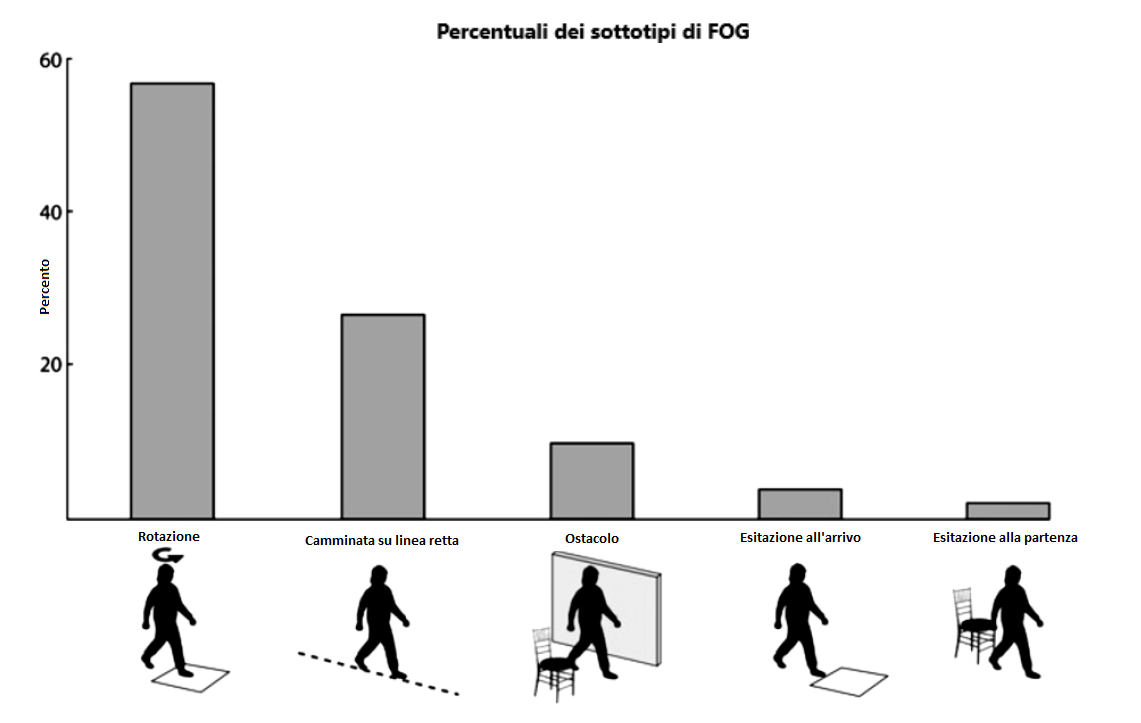
\includegraphics[scale=0.4]{images/Proportion_of_FOG_sub-types.png}
	\caption{Diversi tipi di Freezing esistenti e loro percentuale di incidenza su un certo gruppo di malati di Parkinson. [Fonte: J.M. Shine et al., 2012]}
\end{figure}
Dallo studio di Schaafsma et al.\cite{30} emerge che gli episodi di Freezing possono anche essere suddivisi in ulteriori tre sottotipi andando ad osservare i movimenti delle gambe dei pazienti e applicando la classificazione di Thompson e Marsden (1995):
\begin{enumerate}
	\item FoG associato a passi molto piccoli e strascicati con il minimo movimento in avanti (trascinamento con piccoli passi);
	\item FoG caratterizzato da tremore alle gambe, ma nessun movimento in avanti efficace (tremito da fermo);
	\item FoG caratterizzato da acinesia completa, vale a dire, nessun movimento osservabile delle gambe.
\end{enumerate}
La necessità di dividere il FoG in sottogruppi dipende dal fatto che questi ultimi potrebbero avere origine differente e quindi essere provocati da cause separate.
\subsection{Influenza del FoG nella camminata}
Il Freezing of Gait influenza il pattern del cammino sia all’inizio della deambulazione sia a regime incrementando o diminuendo in modo evidente i valori dei parametri sopra riportati. Ad esempio, nei parkinsoniani che manifestano frequenti fenomeni di Freezing, la variabilità della durata del passo risulta maggiore e la lunghezza del passo minore rispetto alle situazioni in cui il Freezing è assente. Inoltre, la velocità e la lunghezza dei primi tre passi sono significativamente inferiori nei pazienti con malattia di Parkinson e con Freezing rispetto ai soggetti sani. Anche se il Freezing è tipicamente considerato un problema motorio, il fatto che spesso compaia quando il paziente si trova in spazi ristretti, suggerisce che la percezione dello spazio contribuisce in larga misura a scatenare il sintomo\cite{37}.Inoltre, i pazienti con Freezing hanno velocità media del cammino minore rispetto a pazienti sani e subiscono una riduzione ulteriore della velocità nel momento in cui si trovano a dover attraversare una porta o uno spazio stretto. Depressione e ansia possono comportare un carico cronico sulla salute mentale, e la depressione è associata con i cambiamenti di andatura, tra cui una maggiore variabilità passo-a-passo. Il Dual-Tasking, l’ansia e la depressione possono incrementare la variabilità del passo, la di-sincronizzazione di gamba destra e sinistra e l'asimmetria nei pazienti con Parkinson riducendo così la soglia per il FoG. \\
\begin{figure}[]
	\centering
	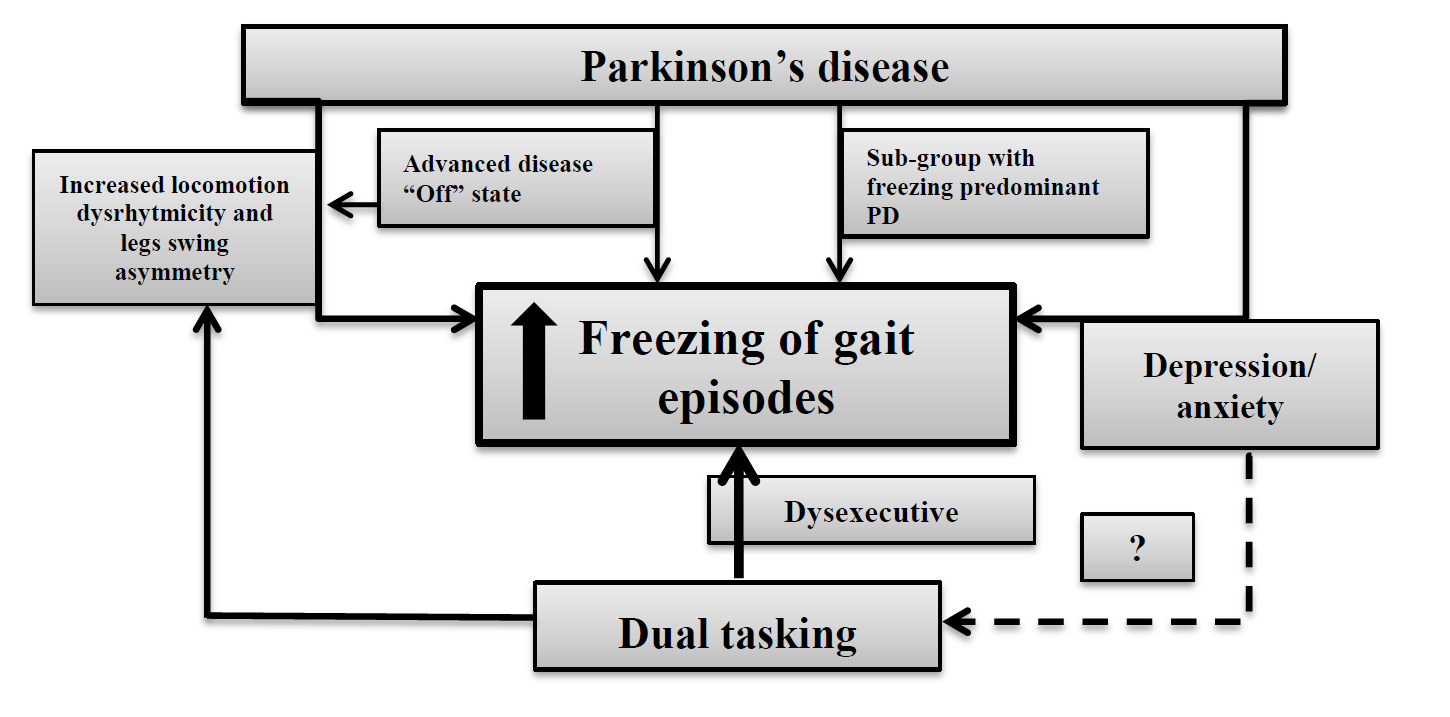
\includegraphics[scale=0.4]{images/Schema_Concettuale_Stress.png}
	\caption{Quadro concettuale relativo al Freezing of Gait (FoG) riguardante aspetti mentali e motori.}
\end{figure}

\section{Machine Learning}
